\begin{pastexam}[label={px:ntust-110-ice-06}]{臺科大資工所 110 學年度 第 6 題}
（問答）

Answer the following questions. (28\%)
\begin{enumerate}[label=(\alph*)]
\item Give the prefix expression for the following expression. (3\%)
\begin{quote}A*(B+C)/D-E\end{quote}
\item What is the post-order traversal of the following tree? (4\%)

\begin{center}
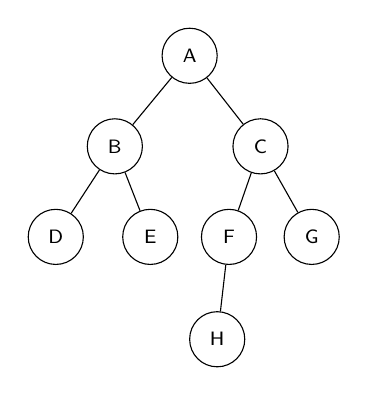
\begin{tikzpicture}[x=1cm,y=1cm,every node/.style={circle,draw,inner sep=0pt,minimum size=7mm,font=\sffamily\scriptsize}]
\node (A) at (0,0) {A};
\node (B) at (-0.95,-1.15) {B};
\node (C) at (0.9,-1.15) {C};
\node (D) at (-1.7,-2.3) {D};
\node (E) at (-0.5,-2.3) {E};
\node (F) at (0.5,-2.3) {F};
\node (G) at (1.55,-2.3) {G};
\node (H) at (0.35,-3.6) {H};
\draw (A)--(B) (A)--(C) (B)--(D) (B)--(E) (C)--(F) (C)--(G) (F)--(H);
\end{tikzpicture}
\end{center}
\item What is the minimum and maximum number of nodes in a complete binary tree of height h? (6\%)
\item Draw the binary min heap that results from inserting 12, 9, 14, 16, 4, 17, 6, 8, 2 in that
order into an initially empty binary heap. Draw the final tree. (10\%)
\item Remove the first two smallest values from the heap created in (d) and reconstruct the min
heap. Draw the resulting tree. (5\%)
\end{enumerate}
\end{pastexam}

\begin{pastsoln}
答案：(a) \texttt{- / * A + B C D E}；(b) D E B H F G C A；(c) 最少 $2^{h-1}$、最多 $2^h - 1$ 個（單一節點
高度為 $1$）；(d)(e) 見下面的圖。

\textbf{(a)} $*$、$/$ 同級由左往右結合，又都比 $-$ 高，所以式子是 $\bigl((A*(B+C))/D\bigr)-E$。 運算式樹
的根是 $-$，左子樹是 $(A*(B+C))/D$，右子樹是 $E$。 前序（根、左、右，資結書第~6.3.5~節）逐層展開：
\[
\begin{aligned}
&{-}\ [\,(A*(B+C))/D\,]\ E \\
={}&{-}\ {/}\ [\,A*(B+C)\,]\ D\ E \\
={}&{-}\ {/}\ {*}\ A\ [\,B+C\,]\ D\ E \\
={}&{-}\ {/}\ {*}\ A\ {+}\ B\ C\ D\ E.
\end{aligned}
\]
把它當前序式求值檢查：$+\,B\,C$ 是 $B+C$；$*\,A\,(B+C)$ 是 $A*(B+C)$；$/\,(\ldots)\,D$；最後 $-\,(\ldots)\,E$，
和原式相同。

\textbf{(b)} 後序是「左子樹、右子樹、根」（資結書第~7.3~節）。 $B$ 的子樹：D、E、B。 $C$ 的子樹：$F$ 的
子樹是 H、F（$F$ 只有一個子節點 $H$，不管 $H$ 在左邊還是右邊，後序都是 H 再 F），然後 G，最後 C。 最後是根 A：
\[
\text{D E B H F G C A}.
\]

\textbf{(c)} 採用資結書的定義：只有一個節點的樹高度是 $1$。 完整二元樹的前 $h - 1$ 層全滿，第 $h$ 層從左邊
連續放（資結書第~7.1~節）。
\begin{itemize}
\item 最多：第 $h$ 層也全滿，是完美二元樹，$1 + 2 + \cdots + 2^{h-1} = 2^h - 1$ 個（資結書定理~7.1 的上界）。
\item 最少：前 $h - 1$ 層全滿共 $2^{h-1} - 1$ 個，第 $h$ 層至少要有一個（否則高度只有 $h - 1$），共
$2^{h-1}$ 個。
\end{itemize}
所以 $2^{h-1} \le n \le 2^h - 1$，等價於 $h = \lfloor \lg n \rfloor + 1$（資結書定理~7.3）。 如果高度從 $0$
算（單一節點高度 $0$），把 $h$ 換成 $h + 1$：最少 $2^h$、最多 $2^{h+1} - 1$。 作答時寫出採用哪一種定義。

\textbf{(d)} 每次插入放在最後一格再上浮（資結書第~8.1.5~節，最小堆積版）。 每列是插入之後的陣列，位置從
$1$ 開始：
\begin{center}
\small
\begin{tabular}{lc*{9}{c}}
\toprule
插入 & 交換 & 1 & 2 & 3 & 4 & 5 & 6 & 7 & 8 & 9 \\
\midrule
12 & 0 & 12 \\
9 & 1 & 9 & 12 \\
14 & 0 & 9 & 12 & 14 \\
16 & 0 & 9 & 12 & 14 & 16 \\
4 & 2 & 4 & 9 & 14 & 16 & 12 \\
17 & 0 & 4 & 9 & 14 & 16 & 12 & 17 \\
6 & 1 & 4 & 9 & 6 & 16 & 12 & 17 & 14 \\
8 & 2 & 4 & 8 & 6 & 9 & 12 & 17 & 14 & 16 \\
2 & 3 & 2 & 4 & 6 & 8 & 12 & 17 & 14 & 16 & 9 \\
\bottomrule
\end{tabular}
\end{center}
插入 $9$：放在位置 $2$，父節點 $12$ 比它大，交換。 插入 $4$：放在位置 $5$，父節點 $A[2] = 12$ 比它大，交換；再和根 $9$ 交換。
插入 $6$：放在位置 $7$，父節點 $14$ 比它大，交換；父節點 $4$ 比它小，停。
插入 $8$：放在位置 $8$，和父節點 $16$、再和 $9$ 交換，父節點 $4$ 比它小，停。 插入 $2$：位置 $9$ 往上的
父節點依序是 $A[4] = 9$、$A[2] = 8$、$A[1] = 4$，都比它大，交換三次，$2$ 到根。 最後的樹是下圖 (a)。

\textbf{(e)} 每次取出最小值：把最後一格搬到根，再往下和較小的子節點交換（下沉，資結書虛擬碼~8.2）。
\begin{itemize}
\item 取出 $2$：最後一格的 $9$ 搬到根，和較小的子節點 $4$ 交換，到了位置 $2$；子節點 $8, 12$ 中 $8$ 比它小，
交換，到了位置 $4$；子節點只剩 $16$，比它大，停：$\langle 4, 8, 6, 9, 12, 17, 14, 16 \rangle$。
\item 取出 $4$：最後一格的 $16$ 搬到根，和較小的子節點 $6$ 交換，到了位置 $3$；子節點 $17, 14$ 中 $14$ 比它小，
交換，到了位置 $7$，沒有子節點，停：$\langle 6, 8, 14, 9, 12, 17, 16 \rangle$，是下圖 (b)。
\end{itemize}
\begin{center}
\begin{minipage}{0.5\linewidth}\centering
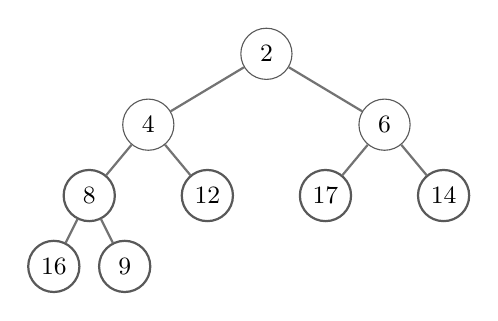
\begin{tikzpicture}[level distance=9mm,
  every node/.style={circle,draw=black!65,minimum size=6.5mm,inner sep=0pt,font=\small},
  edge from parent/.style={draw=black!55,thick},
  level 1/.style={sibling distance=30mm},
  level 2/.style={sibling distance=15mm},
  level 3/.style={sibling distance=9mm}]
\node {2}
  child {node {4}
    child {node {8}
      child {node {16}}
      child {node {9}}}
    child {node {12}}}
  child {node {6}
    child {node {17}}
    child {node {14}}};
\end{tikzpicture}

{\footnotesize (a) (d) 的答案}
\end{minipage}\hfill
\begin{minipage}{0.45\linewidth}\centering
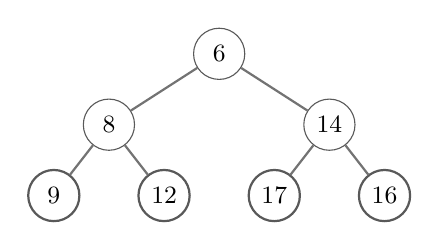
\begin{tikzpicture}[level distance=9mm,
  every node/.style={circle,draw=black!65,minimum size=6.5mm,inner sep=0pt,font=\small},
  edge from parent/.style={draw=black!55,thick},
  level 1/.style={sibling distance=28mm},
  level 2/.style={sibling distance=14mm}]
\node {6}
  child {node {8}
    child {node {9}}
    child {node {12}}}
  child {node {14}
    child {node {17}}
    child {node {16}}};
\end{tikzpicture}

\vspace{9mm}
{\footnotesize (b) (e) 的答案}
\end{minipage}
\end{center}
\end{pastsoln}
